\chapter{Extra functionality} \label{sec:extra_func}

\section{User friendly GUI} 
A user friendly GUI was implemented in order to report important measurements in a readable format, voltage, current and phase measurements were routinely sampled as can be seen in Figure \ref{subfig:python_code_flow}, and these measurements were added to an array with a running window approach. Real and reactive total power usage was calculated with Formulas \ref{eq:realpower} and \ref{eq:reactivepower}, and to display the energy usage in Wh and Varh Equations \ref{eq:realpowere} and \ref{eq:reactivepowere} were applied to the calculated real and reactive power values every second. The graphs and GUI data was updated every second for live time data displaying whilst not interfering with the basic functionality introduced in Chapter \ref{ch:reporting}.

\begin{align}
  P &= V_{rms}I_{rms}cos(\phi) \label{eq:realpower} \\
  Q &= V_{rms}I_{rms}sins(\phi) \label{eq:reactivepower} \\
  E &= T\sum_{i=0}^{N-1} P(nT)\label{eq:realpowere} \\
  E &= T\sum_{i=0}^{N-1} Q(nT)\label{eq:reactivepowere} 
\end{align}

\begin{figure}[ht]
 \footnotesize
 \centering
    \begin{subfigure}[]{0.45\textwidth}
              \centering
  		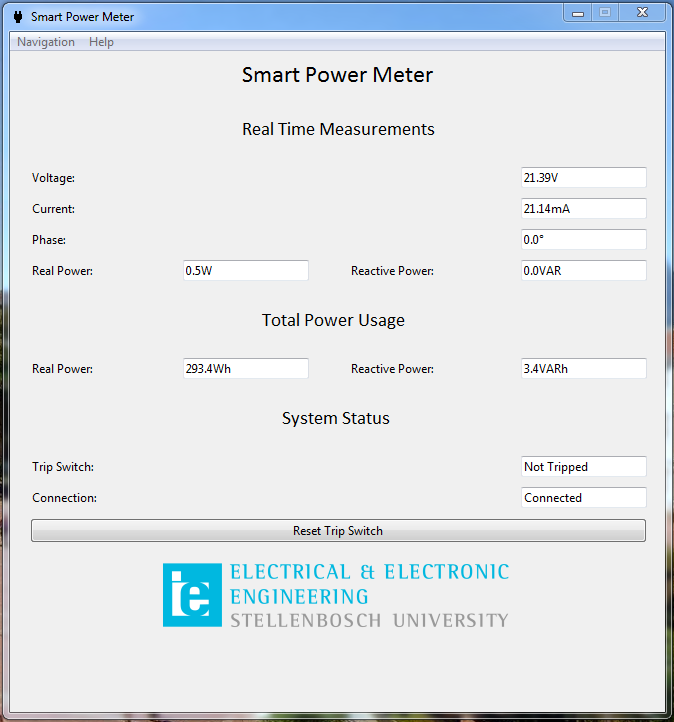
\includegraphics[width=1.0\linewidth]{./Figures/gui_home.PNG}
		    \caption{} \label{subfig:gui_home}
     \end{subfigure}
     \begin{subfigure}[]{0.45\textwidth}
             \centering
  		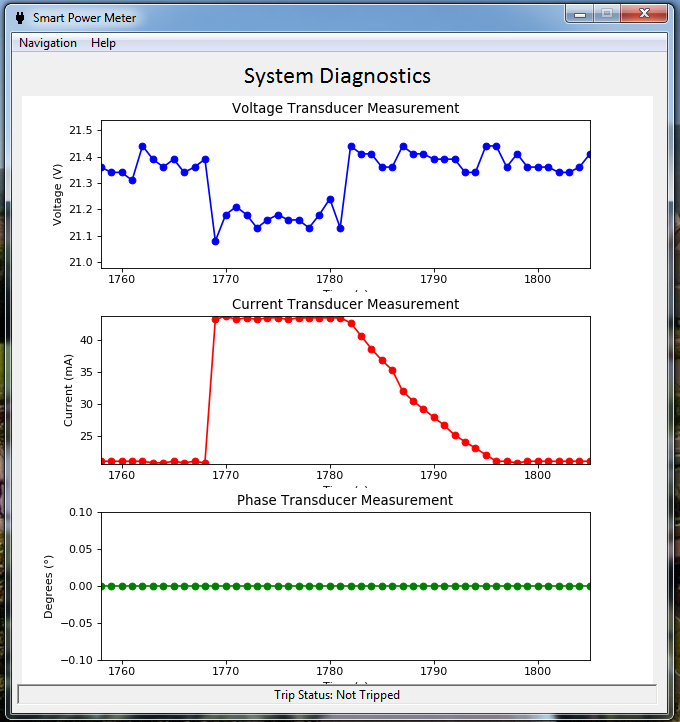
\includegraphics[width=1.0\linewidth]{./Figures/gui_meas.PNG}
		   \caption{ } \label{subfig:gui_meas}
     \end{subfigure}
     \caption[Improved Graphical User Interface.]{Improved Graphical User Interface. (a) Home Screen. (b) Measurements Screen.} \label{fig:gui_extra_results}
\end{figure}

\section{SR latch analogue initialisation} 
To ensure that the load received power on startup conditions where the Arduino was not connected first an analogue initialisation circuit was created to define the state of the SR latch. This circuit design can be seen in Figure \ref{subfig:switch_init_schem}, the thought process behind this design is that on startup the capacitor holds no charge and $v_{ref}$ is thus at ground, meaning that the transistor is switched off and no current will flow into the collector as it is an open-circuit. The resistor $R_{11}$ thus has no voltage drop across it and the voltage at the collector of the transistor will be equal to that of the 5V rail. As the capacitor charges up the transistor switches on, and the value of reset drops to $V_{CE(sat)}=0.2V$, which is a logical low. The simulation documenting this process can be seen in Figure \ref{subfig:switch_init_meas}.
\begin{figure}[ht]
 \footnotesize
 \centering
    \begin{subfigure}[]{0.45\textwidth}
              \centering
  		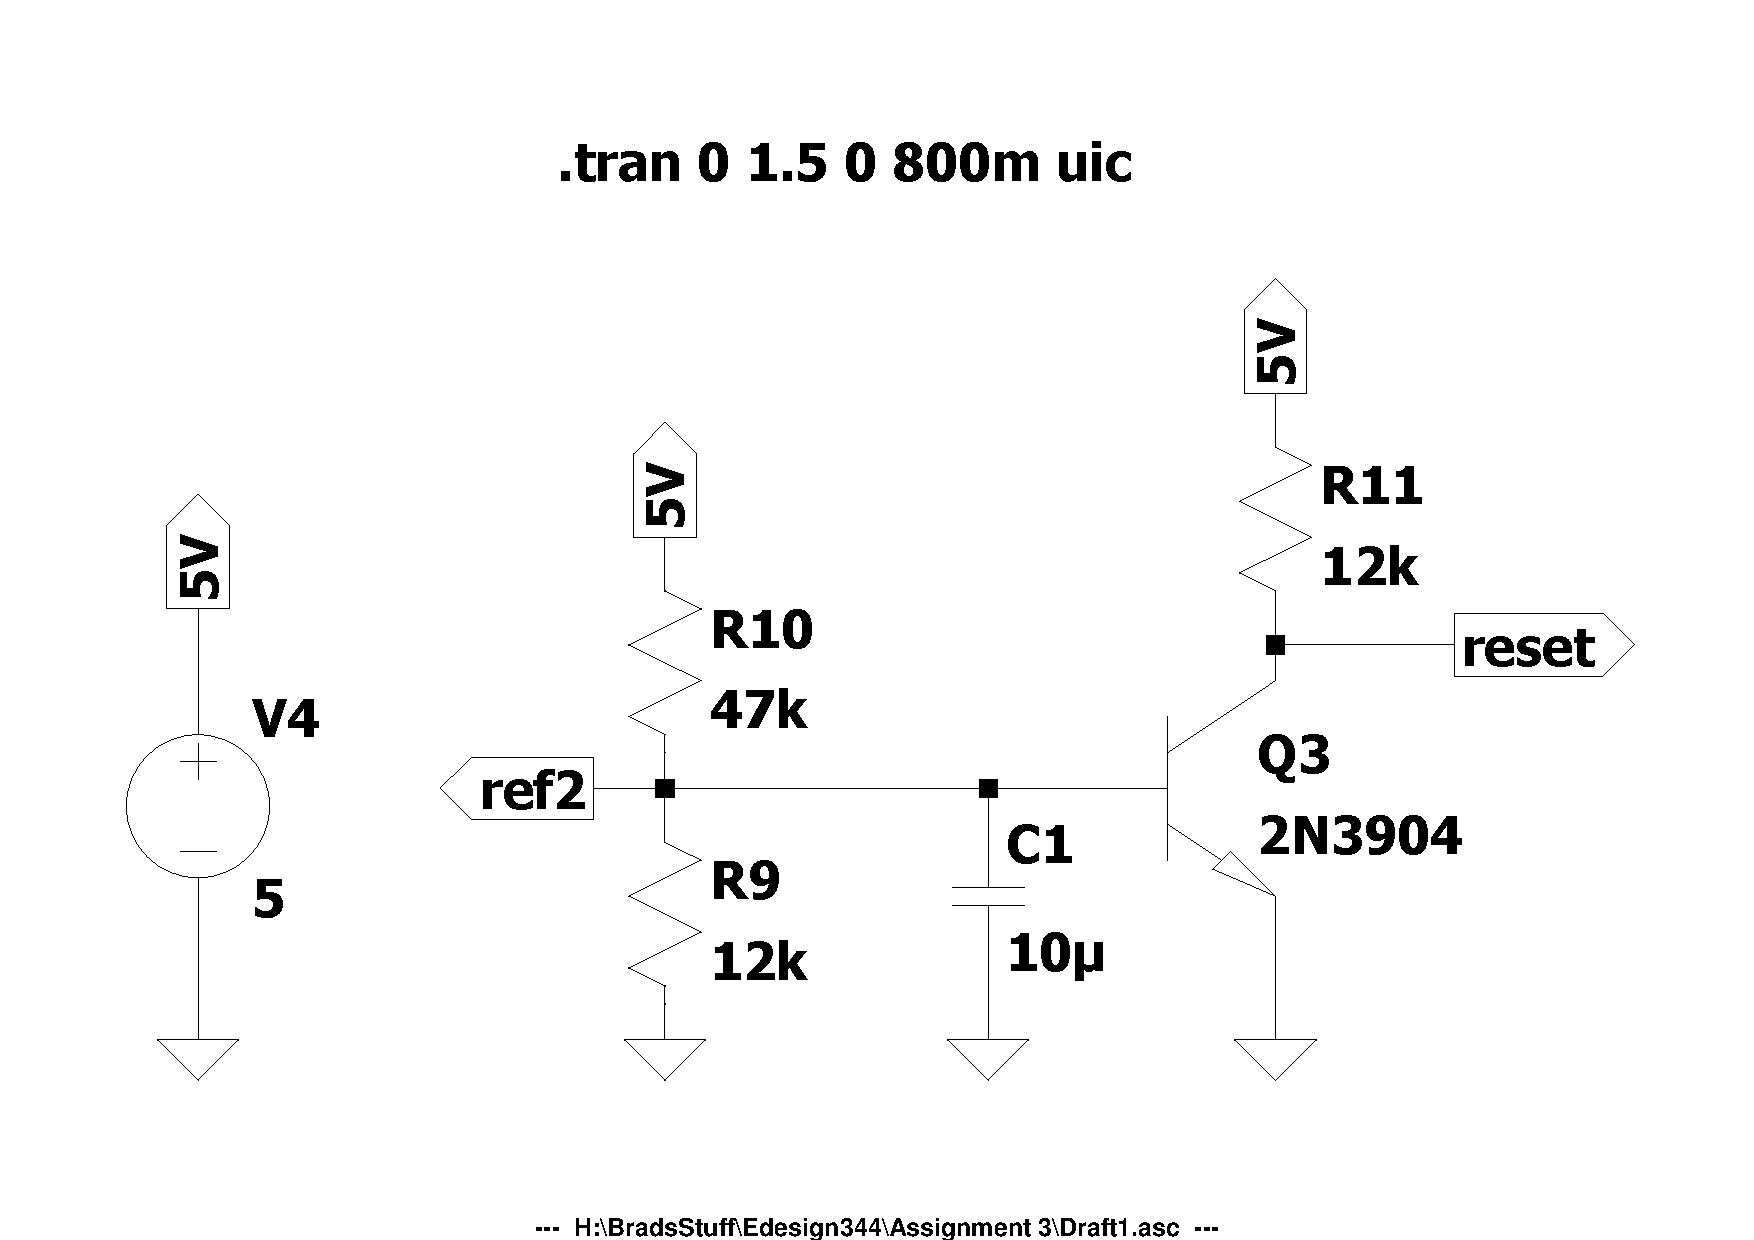
\includegraphics[width=1.0\linewidth]{./Figures/reset_init_schem.pdf}
		    \caption{} \label{subfig:switch_init_schem}
     \end{subfigure}
     \begin{subfigure}[]{0.45\textwidth}
             \centering
  		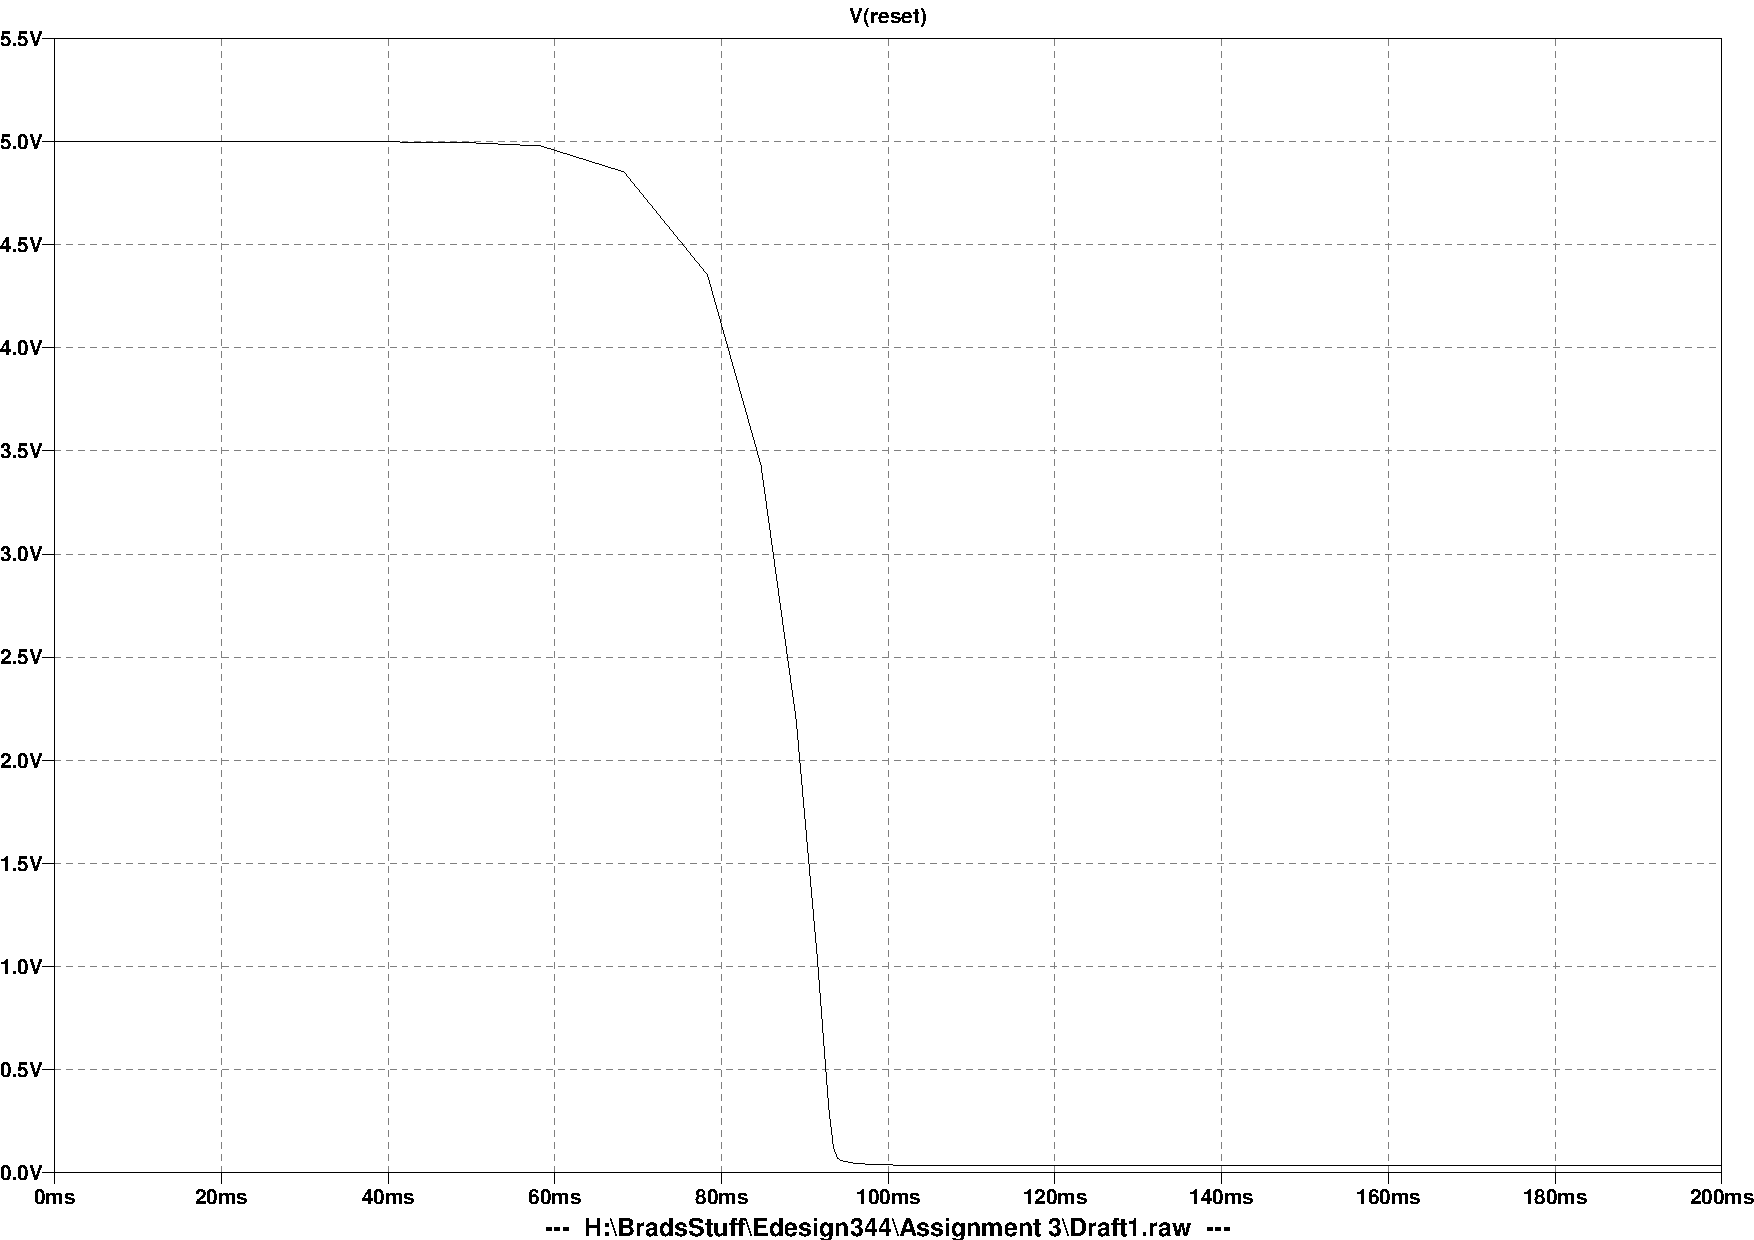
\includegraphics[width=1.0\linewidth]{./Figures/reset_init_output.pdf}
		   \caption{ } \label{subfig:switch_init_meas}
     \end{subfigure}
     \caption[Initialisation circuitry for the SR latch.]{Initialisation circuitry for SR latch. (a) Circuit Diagram. (b) Output signal measurement. } \label{fig:switch_extra_results}
\end{figure}

\section{Status LEDs} 
Two status LEDs were added to the system, where one was used to display whether the board received power, and another LED displayed whether the trip switch was active. The power status LED received was powered from the -5V rail, and as the -5V rail could only work with the Arduino connected, it served a dual purpose of displaying whether the Arduino was initialised correctly.